% L13a figure: one HTTP request and its response, with the parts labeled.
%
% Left: the request that asks the National Weather Service API for the data it
% holds about Ithaca, NY. Right: the response, shortened to two headers and a
% few fields of the body. The text is a real exchange captured November 12, 2026.
% Blue marks the method and the status code.
%
% Drawn on November 12, 2026 with the palette and build of the L12c figures.
% The notebook SVG carries a dark palette added by theme_svg.py; keep new colors
% in that script's mapping when changing the palette here.
\documentclass[tikz,border=4pt]{standalone}
\usepackage[no-math]{fontspec}
\IfFontExistsTF{Arial}{\setsansfont{Arial}}{\setsansfont{TeX Gyre Heros}}
\IfFontExistsTF{Menlo}{\setmonofont{Menlo}[Scale=0.88]}{}
\renewcommand{\familydefault}{\sfdefault}
\usepackage{amsmath,amssymb}
\usetikzlibrary{arrows.meta, calc, fit, backgrounds, positioning, decorations.pathreplacing}

% Ink, blue, gray, and band match the L12c figures.
\definecolor{vnink}{HTML}{202124}
\definecolor{gdblue}{HTML}{0091FF}
\definecolor{gdgray}{HTML}{6D7278}
\definecolor{waband}{HTML}{EEF0F2}
\definecolor{nodefill}{HTML}{FFFFFF}

\begin{document}
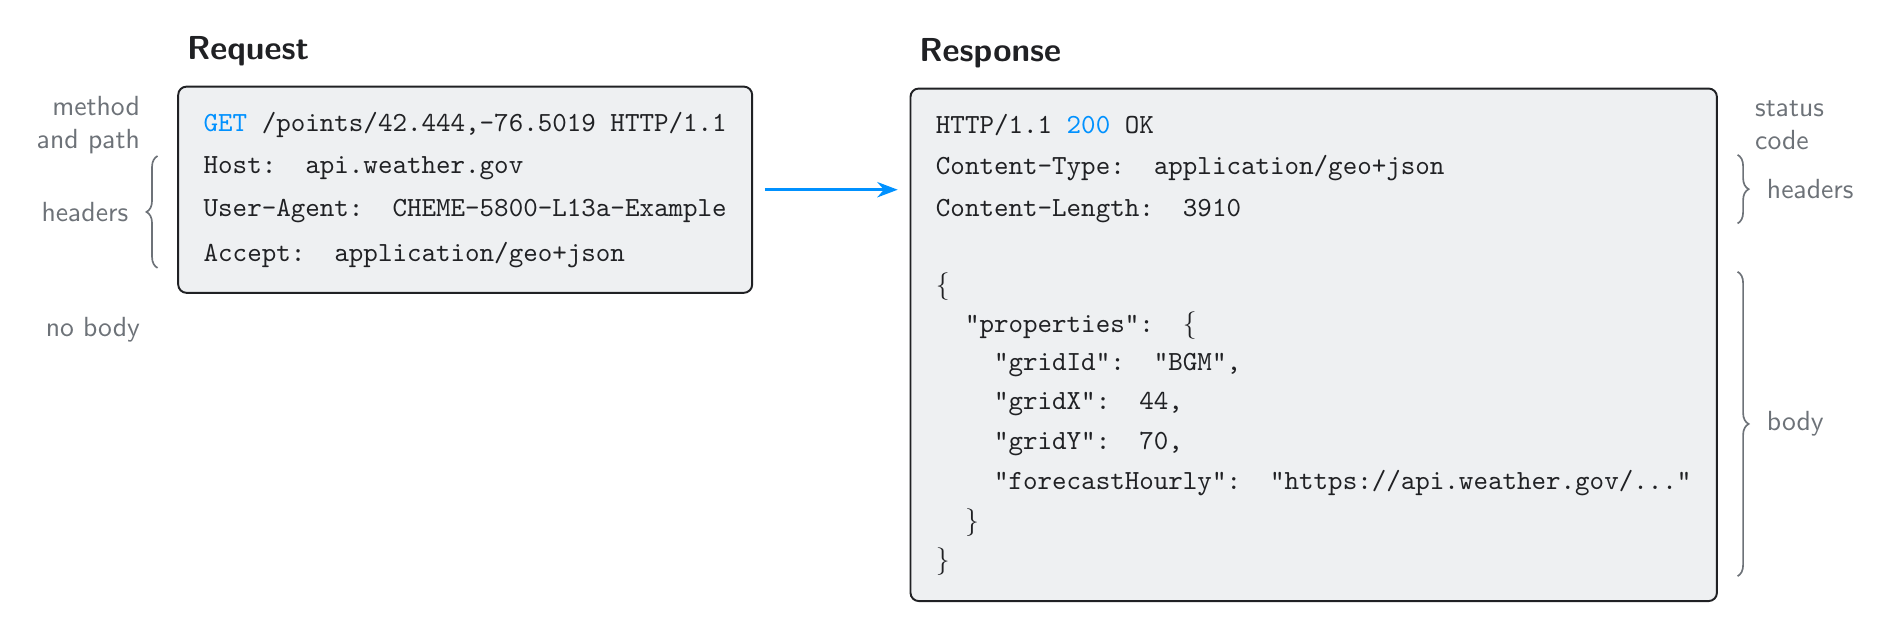
\begin{tikzpicture}[
  font=\sffamily\large,
  ln/.style={anchor=west, font=\ttfamily\normalsize, text=vnink, inner sep=0pt},
  panel/.style={draw=vnink, rounded corners=3pt, fill=waband, line width=0.7pt, inner sep=9pt},
  title/.style={font=\sffamily\large\bfseries, text=vnink, anchor=south west},
  part/.style={font=\sffamily\normalsize, text=gdgray, align=right},
  partr/.style={font=\sffamily\normalsize, text=gdgray, align=left},
  br/.style={decorate, decoration={brace, amplitude=4pt}, draw=gdgray, line width=0.6pt}
]
\newcommand{\hl}[1]{\textcolor{gdblue}{\bfseries #1}}

% ------------------------------------------------------------------ the request
\node[ln] (r1) at (0, 0.00)  {\hl{GET} /points/42.444,-76.5019 HTTP/1.1};
\node[ln] (r2) at (0,-0.55)  {Host: api.weather.gov};
\node[ln] (r3) at (0,-1.10)  {User-Agent: CHEME-5800-L13a-Example};
\node[ln] (r4) at (0,-1.65)  {Accept: application/geo+json};
\begin{scope}[on background layer]
  \node[panel, fit=(r1)(r2)(r3)(r4)] (req) {};
\end{scope}
\node[title] at ($(req.north west)+(0,0.12)$) {Request};

\node[part, anchor=east] at ($(req.west |- r1)+(-0.35,0)$) {method\\and path};
\draw[br] ($(req.west |- r4.south)+(-0.25,0)$) -- ($(req.west |- r2.north)+(-0.25,0)$)
  node[part, midway, left=7pt] {headers};
\node[part, anchor=east] at ($(req.west |- r4)+(-0.35,-0.95)$) {no body};

% ----------------------------------------------------------------- the response
\node[ln] (s1)  at (9.3, 0.00) {HTTP/1.1 \hl{200} OK};
\node[ln] (s2)  at (9.3,-0.55) {Content-Type: application/geo+json};
\node[ln] (s3)  at (9.3,-1.10) {Content-Length: 3910};
\node[ln] (s4)  at (9.3,-2.05) {\{};
\node[ln] (s5)  at (9.3,-2.55) {\ \ "properties": \{};
\node[ln] (s6)  at (9.3,-3.05) {\ \ \ \ "gridId": "BGM",};
\node[ln] (s7)  at (9.3,-3.55) {\ \ \ \ "gridX": 44,};
\node[ln] (s8)  at (9.3,-4.05) {\ \ \ \ "gridY": 70,};
\node[ln] (s9)  at (9.3,-4.55) {\ \ \ \ "forecastHourly": "https://api.weather.gov/..."};
\node[ln] (s10) at (9.3,-5.05) {\ \ \}};
\node[ln] (s11) at (9.3,-5.55) {\}};
\begin{scope}[on background layer]
  \node[panel, fit=(s1)(s2)(s3)(s4)(s5)(s6)(s7)(s8)(s9)(s10)(s11)] (res) {};
\end{scope}
\node[title] at ($(res.north west)+(0,0.12)$) {Response};

\node[partr, anchor=west] at ($(res.east |- s1)+(0.35,0)$) {status\\code};
\draw[br] ($(res.east |- s2.north)+(0.25,0)$) -- ($(res.east |- s3.south)+(0.25,0)$)
  node[partr, midway, right=7pt] {headers};
\draw[br] ($(res.east |- s4.north)+(0.25,0)$) -- ($(res.east |- s11.south)+(0.25,0)$)
  node[partr, midway, right=7pt] {body};

% --------------------------------------------- the request goes out, the response comes back
\draw[->, >={Stealth[length=2.6mm]}, line width=1.0pt, draw=gdblue]
  ($(req.east)+(0.15,0)$) -- ($(res.west |- req.east)+(-0.15,0)$);

\end{tikzpicture}
\end{document}
